\RequirePackage[l2tabu, orthodox]{nag}

\documentclass[11pt,a4paper]{book}

\usepackage[english]{babel}
\usepackage[T1]{fontenc}
\usepackage[utf8]{inputenc}

\usepackage{microtype}
\usepackage{mathtools}
\usepackage{todonotes}
\usepackage{graphicx}
\usepackage{blindtext}
\usepackage[hidelinks]{hyperref}
\usepackage{pdfpages}
\usepackage{fullpage}

\usepackage{csquotes}
\usepackage{booktabs}
\usepackage{standalone}
\usepackage{amssymb}

\usepackage{tcolorbox}
\tcbuselibrary{listingsutf8,breakable,theorems,skins}
%The paper size for this thesis is the Swedish format s5
\usepackage[
    binary-units=true,
    separate-uncertainty=true,
    uncertainty-separator={\pm}
    ]
{siunitx}
\usepackage{lmodern}
\usepackage{verbatim}
\usepackage{todonotes}
\usepackage{subcaption}
\usepackage[standard]{ntheorem}
\usepackage{paralist}
\usepackage[noabbrev]{cleveref}
\usepackage{braket}
\usepackage{tipa}
\usepackage{multirow}
\usepackage{textcomp}

\usepackage{caption}

\usepackage{mathptmx}
\usepackage[symbol]{footmisc}
\usepackage{makeidx}
\usepackage{helvet}
\usepackage{tikz}
\usepackage{pgfplots}
\usepackage{rotating}
\usepackage[siunitx]{circuitikz}
\usepackage[section,acronym]{glossaries}
\usepackage[style=numeric-comp,backend=biber,%
    firstinits=true,sorting=none,sortfirstinits=true,clearlang=true,%
    maxnames=3,minnames=1,uniquename=false,%
    maxbibnames=10
]{biblatex}
\usepackage{tablefootnote}
\addbibresource{references.bib}
\graphicspath{{./graphics/}}
\definecolor{theWhite}{gray}{0.9}
\definecolor{theBlack}{gray}{0.2}
\makeindex
\DeclareSIUnit\combustion{c}
\DeclareSIUnit[per-mode=reciprocal]\mgc{\milli\gram\per\combustion}
\DeclareSIUnit{\rpm}{rpm}
\DeclareSIUnit{\RON}{RON}


%% If the following definition throws an error, you'll need a newer version of your
% Latex distribution (from at least the second half of 2013)
\newtcbinputlisting[]{\commandline}[2][]{%
    oversize,
    colback=theBlack,
    colframe=red!50!white,
    coltext=theWhite,
    listing only,
    listing options={language={bash},aboveskip=0pt,belowskip=0pt,nolol,
    basicstyle=\ttfamily\bfseries,extendedchars=true},
    enhanced,
    breakable,
    lines before break=4,
    listing file={#2},
    arc=8pt,
    #1
}

\newtcbinputlisting[]{\tcbexample}[2][]{%
    oversize,
    colframe=green!50!white,
    text only,
    enhanced,
    breakable,
    lines before break=4,
    listing file={#2},
    arc=8pt,
    #1
}

\newcommand{\Mfig}[1]{%
\begin{figure}
    \centering
    \missingfigure{#1}
    \caption{#1}
\end{figure}}


\tikzstyle{startstop} = [rectangle, rounded corners, minimum width=3cm, minimum height=1cm,text centered, draw=black, fill=red!30]
\tikzstyle{io} = [trapezium, trapezium left angle=70, trapezium right angle=110, minimum width=3cm, minimum height=1cm, text centered, draw=black, fill=blue!30]
\tikzstyle{process} = [rectangle, minimum width=3cm, minimum height=1cm, text centered, draw=black, fill=orange!30]
\tikzstyle{small} = [circle, minimum width=1cm, minimum height=1cm, text
centered, draw=black, fill=orange!10]
\tikzstyle{decision} = [diamond, minimum width=3cm, minimum height=1cm, text centered, draw=black, fill=green!30]

\usetikzlibrary{shapes.geometric, arrows}


\begin{document}

\title{Trionic 7 Documentation}
\author{Dilemma, typeset in \LaTeX by Jonathan Jogenfors}

\maketitle
\clearpage
\frontmatter
\chapter{Introduction}
This document is intended for Saab fanatics and engineers who want to start
understanding the Saab Trionic 7 motor management system. It will give as much
information as possible about the technical part of the system. The only
limitation will be the knowledge of the author. In short the content of this
document will enable you to understand Trionic 7 better and give you hands-on
information about altering the maps it uses. Prerequisites are minor electronics
and computer knowledge and of course some understanding of how a turbo charged
engine works. Throughout the document the T7Suite software will be referenced.
This software will enable you to really \enquote{get into} the Trionic. The T7Suite
software can be downloaded from the T7Suite website.

\chapter{Acknowledgements}
This document is the result of contributions and hard work from many people over
a long time. Version 1.0 was put together by Dilemma in 2010, and he thanks
people on ecuproject for all their help. Dilemma gives special thanks go to General
Failure, J.K. Nilsson, Hook, Hma, Vigge, Mackan, Sandy Rus, JKB, L4staero and
Steve Hayes. Big thanks to solving the checksum calculation, I-bus information,
and P-bus information goes to Tomili and General Failure. L4staero contributed
information on the secondary lambda sensor. Magnus Lirell and David Goncalves
contributed information to the SID text and automatic transmission Canbus
message formats. David Concalves contributed information on the SID text
priority and Audio RDS Canbus message formats.

Beginning in 2015, a rework was started by Jonathan Jogenfors (Etnoy) to typeset
the information using \LaTeX{} and update the information together with other
enthusiasts over at TrionicTuning. Special thanks to chriva and many others.
This project is ongoing and you can check out the current status of the project
at \url{https://github.com/etnoy/t7ref}.

\chapter{Changelog}
\section*{From version 1.0 to 2.0}
Version 1.0 of this document is popularly referred to as
\enquote{\texttt{Trionic7.pdf}} as that was the filename. This is the version
produced by Dilemma and written mainly in Microsoft Word. As the original .doc
files appear to have been lost version 2.0 was created using \LaTeX{}. As a part
of this project, several appendices had to be removed due to copyright reasons.
A reader interested in finding that information is better off reading the actual
technical articles as follows:
\textcite{EstillIntercooler,FerozepuriaTurbocharger,Eriksson1998}.

\listoftodos[Things to be done]
This chapter tracks the todo list for this document. This includes information
that is deemed missing, incorrect, unclear, or needs rework. Also, a lot of
figures and graphs must be manually imported form Dilemma's document, those are
also listed here.


\tableofcontents
\mainmatter
\chapter{Hardware}
The Trionic 7 is built around a Motorola MC68332 (CPU32) microcontroller. This
is a 32-bit controller that handles the entire motor management including fuel
injection, ignition timing and boost pressure control. The processor has a vast
\SI{4}{\mega\byte} (\SI{512}{\kilo\byte}) flash memory for fetching program code
and maps. This flash memory consisting of a AM29F400BT-90SI (AMD) holds the
program memory. There is a coprocessor from Philips, a P83C592FHA/019. This is a
8-bit 8051-based microcontroller with a CAN (Controller Area Network) module. As
the CAN physical line driver there is an Intel AN82527 (same family as used in
Trionic 5). RAM memory is done by two \SI{32}{\kilo\bit} SRAM chips
(U62H256S1K). There is also a special component that would appear to be a
barometric pressure sensor.

\section{Integrated Circuit List}
The table below lists almost all integrated circuits on the board. This is just to give you an idea on what to expect.

\begin{table}
    \centering
    \begin{tabular}{llll}
        Partnumber & Function & Usage & \# on board \\
        \midrule
        TC55257DFI-85L & SRAM & (working memory) & 1 \\
        16233970 & Microcontroller & Main 32-bit CPU & 1 \\
        PC83C592 & Microcontroller with CAN contr.& 8-bit coprocessor & 1 \\
        AM29F400 & Flash memory & \SI{4}{\mega\bit} & 1 \\
        51862 & DA converter & & 1 \\
        AN82527 & CAN controller    CAN line driver & 1 \\
        16238669 0H11 & Pressure sensor? & &  1
    \end{tabular}
    \caption{}
    \label{tab:}
\end{table}

\section{Block Schematic Diagram}
\begin{figure}[]
    \centering
    \missingfigure{}
    \caption{}
    \label{fig:}
\end{figure}

\section{DI Cassette}
The DI cartridge has a trigger input for firing the four individual sparkplugs. These are triggered by
signals from the ECU on pin 9, 10, 11 and 12 which are generated in the power driver IC CA3236 on
the Trionic PCB (topside, 16 pin DIL housing). Internally these four pins are connected as shown in
the table and the image below.

\begin{table}
    \centering
    \begin{tabular}{cccc}
        DI cartridge pin & ECU pinnumber &  CA3236 pinnumber &  Description \\
        \midrule
        2 & 7 & 1 (OUT A) & Trigger cylinder 1 \\
        3 & 8 & 3 (OUT B) & Trigger cylinder 2 \\
        4 & 67 & 6 (OUT C) & Trigger cylinder 3 \\
        5 & 68 & 8 (OUT D) & Trigger cylinder 4 \\
    \end{tabular}
    \caption{}
    \label{tab:}
\end{table}

\chapter{Flashing}
The Trionic 7 ECU binary images uses several checksums to verify integrity. Most
of them have been easy to figure out, but one of them is so complicated, that it
seems to been done to deter map changing. There are still some unknowns, that
would be nice to figure out. For example, I've discovered some binaries don't
seem to have all four checksums. And of course there could be more checksums
that have gone unnoticed. Two of the checksums are in the end of the binary and
the other two are scattered in the code. The latter ones can be found by using
pattern searching. Again the calculations are pretty simple, and even the harder
checksum is easy to implement.

\section{Checksums}
First of all, there are four different checksums. They have been given names by
Tomi\todo{Who is this?}: \texttt{FB}\index{FB checksum} checksum,
\texttt{F2}\index{F2 checksum} checksum,
\texttt{Misc} checksum\index{Misc checksum}, and \texttt{Area 70000}
checksum\index{Area 7000 checksum}.

\subsection{FB and F2 checksums}\label{sec:FBF2Checksum}
The first two checksums, \texttt{FB} and \texttt{F2}, can be found at the end of
the binary. This end area has been called the file header (footer would be more
logical). See also \todo{Add reference}chapter Trionic 7 file header. The
\texttt{F2} checksum is not present in all binaries, so be aware of this.
Finding the two other checksums is more of a challenge.

\subsection{Misc checksum}
The Misc checksum resides inline within the code. It is usually found somewhere
between \texttt{0x02000} and \texttt{0x05000}. The checksum address can be found
by pattern searching the bin file using a set of hex values along with mask
bits. If a mask bit is not set, the corresponding hex value does not have to
match. Here are the hex values: \texttt{0x48, 0xE7, 0x00, 0x3C, 0x24, 0x7C,
    0x00, 0xF0, 0x00, 0x00, 0x26, 0x7C, 0x00, 0x00, 0x00, 0x00, 0x28, 0x7C,
    0x00, 0xF0, 0x00, 0x00, 0x2A, 0x7C} and the mask is \texttt{1, 1, 0, 0, 0,
0, 1, 1, 1, 1, 0, 0, 0, 0, 1, 1, 1, 1, 0, 0, 0, 0, 1, 1}.

So, we are searching the binary for a string of bytes beginning with
\texttt{0x48, 0xE7, 0x00, 0x3C\ldots}. Then we mask out the bytes that change
from binary to binary. When we've located this pattern, we know where to start.
Now we start primitively disassembling the code. We search for byte patterns
\texttt{0x48, 0x6D}, \texttt{0x48, 0x78}, \texttt{0x48, 0x79}, \texttt{0x2A,
0x7C} and \texttt{0xB0, 0xB9}. The three first patterns reveal addresses and
lengths of checksum areas. There are 15 checksums areas from which the
\texttt{Misc} checksum is calculated. The \texttt{0x2A, 0x7C} pattern gives a
base address for the \texttt{0x48, 0x6D} addresses.

Bear with me. These \texttt{0x2A, 0x7C} addresses are summed with the base
address to make the actual address. This way the address is only 2 bytes long.
On the \texttt{0x48, 0x79} addresses it's 4 bytes long without any base address.
And the \texttt{0x48, 0x78} pattern gives 2 bytes which correspond with the
length of the checksum area. Finally the \texttt{0xB0, 0xB9} pattern is followed
by 4 bytes to the address of the Misc checksum.

\subsection{Area 70000 checksum}
\index{Area 7000 checksum}This checksum refers to an area in the region of
\texttt{0x70000}. Like the \texttt{Misc} checksum, there is no clean way of
finding out the length of the area along with the checksum address. Using
pattern searching with this also has results. There are binaries that are
incompatible with this approach, so this requires some fixing in the future. The
pattern is \texttt{0x20, 0x3c, 0x00, 0x00, 0x11, 0x52, 0x2F, 0x00, 0x20, 0x3C,
    0x00, 0x00, 0x09, 0xD0, 0x2F, 0x00, 0x20, 0x3C, 0x00, 0x00, 0x00, 0xCC,
0xD0, 0x9F} and the mask is \texttt{1, 1, 0, 0, 0, 0, 1, 1, 1, 1, 0, 0, 0, 0, 1,
1, 1, 1, 0, 0, 0, 0, 1, 1}

After finding that pattern, the masked addresses are summed together. In the
pattern, the original addresses are \texttt{0x00001152}, \texttt{0x000009D0} and
\texttt{0x000000CC}. Summing these gives the \texttt{Area 70000} length of
\texttt{0x1BEE}. At the same time this is the address where to find the \texttt{Area
70000} checksum.

\section{Computing the Checksums}
The \texttt{FB} checksum shares the same calculation method as the \texttt{Misc}
and \texttt{Area 70000} checksums. It's simply a sum of the bytes from the
checksum area. Four bytes are made into a 32 bit value and summed with the next
32-bit value. This goes on until there are fewer than 4 bytes left. The last 1,
2 or 3 bytes are then individually summed together with the checksum.

The \texttt{Misc} checksum is a sum of the individual checksums calculated from
15 areas. The checksum calculation used is the same as with the \texttt{FB}
checksum.

Once you have found the length of \texttt{Area 70000}, you can calculate the
checksum by using the function described in \cref{sec:FBF2Checksum}. The start
address is \texttt{0x70000}. Notice that your binary might not have this area
present.

\chapter{Firmware}\index{Firmware}
Once you are done with dumping the flash contents and you want to do more than
only alter variables and maps you can start analyzing the binary. This is a
difficult task because there are a lot of different firmware versions, stock
ones – maybe different per MY and tuned ones that differ for every manufacturer
and stage. In every case the code can be disassembled using a \texttt{6833x}
disassembler like the one in \texttt{IDA Pro}\index{IDA Pro}. There are scripts
available to automatically disassemble the code and make it more readable by
replacing addresses by variable names that are extracted from the symbol
table\index{Symbol table} inside the binary.

\chapter{Symbol table}
Each Trionic 7 firmware file contains a symbol table describing data structures in the
program. The major problem is that from some point in time SAAB started to
compress the symbol tables in the binary file. Probably just to save space in
the flash memory but it has made tuning a little harder. We actually need these
symbol names because they tell us what a certain memory location means. For
unpacked binaries these symbols can be extracted together with their
corresponding memory addresses (ROM and RAM).

\begin{figure}[]
    \centering
    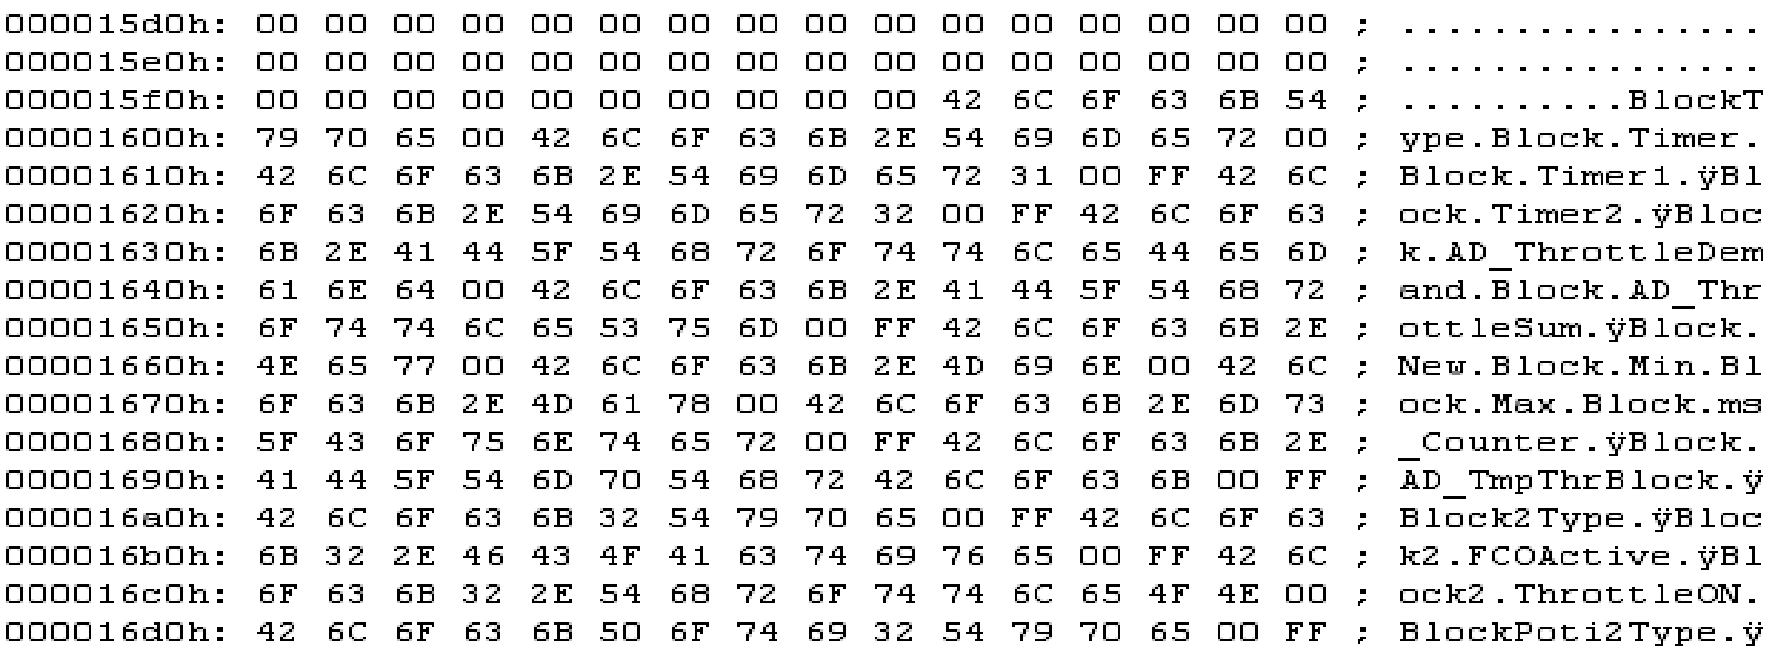
\includegraphics{symboltable.png}
    \caption{}
    \label{fig:}
\end{figure}

While examining the symbol table you can see that the separator is 0x00. In
contrast to T5 where symbol and SRAM addresses reside in the same table, we now
only find the symbol name. In another table in the binary we can find flash
addresses and lengths in the same sequence as the symboltable.

\section{Finding start of symbol table:}

Search binary for string the first sequence of 15 zeros.
\section{Finding start of address lookup table:}
Search binary for 20 00 00 00 XX YY 00 F0 where XX YY is the index of the first
symbol found in the symbollist.

To save you the time to lookup all addresses manually the T7Suite application
will extract all symbol information in one run. Symbol name, flash address and
length will be displayed all together.

This \todo{link}image (6) will give you an idea of what the symbol table should
look like once it has been extracted. See \todo{link}appendix I for a complete
list of known symbols.
\begin{figure}[]
    \centering
    \missingfigure{}
    \caption{}
    \label{fig:}
\end{figure}

When the user double clicks one of the symbols that has a flash address attached
to it, T7Suite will display the corresponding symbol in a viewer. This viewer
will display the data in table form was well as in graphical form.
\begin{figure}[]
    \centering
    \missingfigure{}
    \caption{}
    \label{fig:}
\end{figure}

\chapter{Mapping}
A lot of maps in Trionic 7 are not only made up of a piece of raw data. It also
includes x-axis and y-axis information. T7Suite will automatically display all
known axis information when a map is opened. In Trionic 7 most symbols have an
English name (Trionic 5 has lots of Swedish names) that explains lots about its
function. Also, the symbols are categorized by name, which makes browsing the
symbols much easier. All torque calibration symbols start with
\enquote{TorqueCal.}. T7Suite groups all symbols by their respective category by
default.

\section{Fuel}
Fuel calculation in Trionic 7 is based on the Airmass entering the engine. In
rough steps this seems to be the flow of the calculation:

\begin{enumerate}
    \item Basic calculation of fuel quantity per combustion. The air mass per
        combustion in \si{\milli\gram} is converted to fuel mass in
        \si{\milli\gram} by dividing by the AFR. This is dependent on fuel type:
        \begin{equation}
            \text{mGasoline}=\frac{\text{mAir}}{14.7}, \qquad
            \text{mE85}=\frac{\text{mAir}}{9.765}
        \end{equation}
    \item In case of a cold engine, shortly after starting, rapid load changes,
        knocking or high loads, the fuel mass is multiplied by a compensation
        factor.
    \item The closed loop value is used as a multiplier.
    \item Correction for purge. Multiply by the value for purge adaptation. The
        value is sent to box 5
    \item Long term fuel trim. The fuel mass is multiplied by the multiplicative
        adaptation value.
    \item Additive adaptation. The additive adaptation value is added to the
        fuel mass.
    \item Starting fuel quantity. If the engine has not yet started, starting fuel is
        selected.
    \item The fuel quantity per combustion is the amount of fuel to be
        supplied to the engine.
    \item Computation of injector opening duration. Converts fuel mass to
        opening time from a lookup table.
    \item Injection takes place twice per combustion until the
        camshaft position has been found. Injection duration
        is divided by two.
    \item Battery voltage correction. Injector opening duration is corrected
        by a voltage-dependent factor that is added to the duration.
    \item If fuel cut is active, the computed injector duration is replaced by a
        fuel cut value.
\end{enumerate}
After this computation, the current injector is opened for the computed duration
of time at a determined crank shaft angle. We will now look at the maps that
control the above computation.

The basic fuel quantity is calculated based on air mass (measured from the air
mass flow sensor) and injector constant
(map \texttt{InjCorrCal.InjectorConstant\index{InjCorrCal.InjectorConstant}}).
\begin{figure}
    \centering
    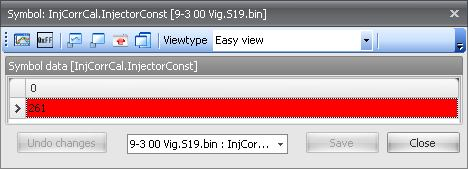
\includegraphics[width=.9\linewidth]{injectorconstant.png}
    \caption{InjCorrCal.InjectorConstant}
    \label{fig:injectorconstant}
\end{figure}
If the engine has reached operating temperature, the standard map
\texttt{BFuelCal.Map} is used. If not, the map is switched out for the cold
start map \texttt{BFuelCal.StartMap}.
\begin{figure}
    \centering
    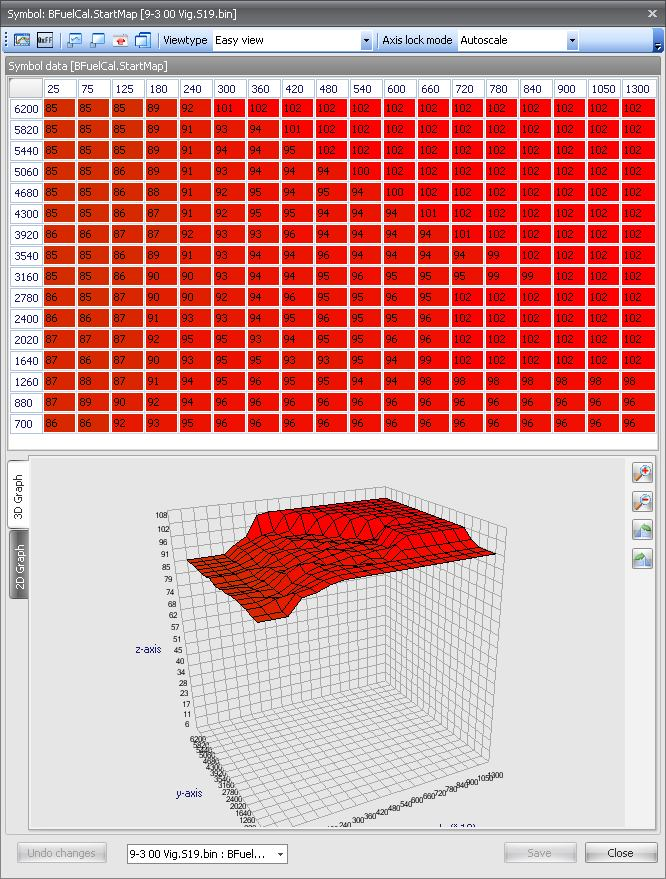
\includegraphics[width=.9\linewidth]{startmap.png}
    \caption{BFuelCal.StartMap}
    \label{fig:startmap}
\end{figure}
\begin{figure}
    \centering
    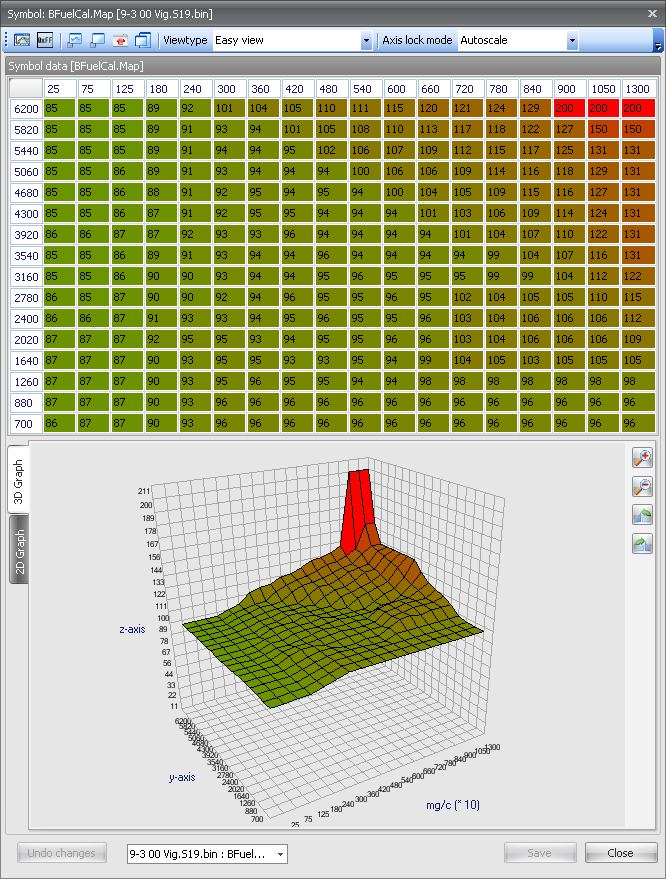
\includegraphics[width=.9\linewidth]{fuelmap.png}
    \caption{BFuelCal.FuelMap}
    \label{fig:fuelmap}
\end{figure}

The areas calibrated to be run in closed loop have a value of \num{1.00(2)}.
Note that the high load part of the maps ramp up to enrich the mixture.
Therefore, adjust the closed loop part of the map first.

To do this, turn closed loop mode off and drive with a wideband lambda sensor.
What you want to achieve is an AFR of 14.7 while driving around under light
loads (i.e. \num{1.00(2)} as per above). What Trionic 7 then does is to compute
an injector duration. If the measured AFR does not achieve the correct value,
the map must be altered. For example, if Trionic 7 computes a duration of
\SI{5}{\milli\second}, a map value of \num{1.1} results in a duration of
$5*1.1=$\SI{5.5}{\milli\second} which means more fuel and a richer mixture.
Conversely, a value below \num{1.1} results in a leaner mixture.

The idea is to get the closed loop area correct first. This will stop any
negative adaption once the tune is finished and allowed to run in closed loop
again. If the closed loop area of your fuel map is too rich it will negatively
adapt over a long period of time. This will have the effect of leaning your
air-fuel ratios across the board.

For example, let's look at a tune with an AFR that is correct in closed loop.
This means that the feedback from the $\textrm O_2$ sensor is enough to
correct the combustion. This can hide a condition where the mixture is too rich
by \SI{13}{\percent} and the $\mathrm O_2$ sensor reduces the fuel mass by
\SI{13}{\percent}. Then, when full power is applied, Trionic 7 enters open loop
mode and the wideband lambda sensor measures an AFR of \num{12.5}.

If this condition remains, Trionic 7 will adjust the long term fuel trim
(multiplicative adaption, \texttt{Amul}\index{Amul}) to be \SI{-13}{\percent}
after a number of weeks. This makes the fuel calculation reduce the fuel
injection by \SI{13}{\percent} over the whole range, including full power.
Here's the danger. At the next full power run, there will be \SI{13}{\percent}
less fuel than ideal, resulting in an AFR of \num{14.0}. The engine now runs
lean and \emph{can fail very quickly, causing massive internal engine damage}.

Now back to fuel mapping. To set closed loop area of fuel map, monitor the AFR
in this light load area and if its wrong after adjusting for large injectors,
start by just adjusting the Injector constant up and down accordingly instead of
altering the closed loop area of the \texttt{BfuelCalMap}. This will affect the
whole map instead of one point. By doing it this way you can almost get AFR spot
on in closed loop area just by a few goes at adjusting the injector constant.

It can be found in \texttt{InjCorrCal.InjectorConst}, the value represents the
injectors flow in mg of fuel (not capacity or cc's as injectors are normally
rated in). The injector constant is a calculation factor used by Trionic 7 to
calculate injection time.

Once closed loop area is done the high load area can be mapped. If its too lean
just increase the values in the relative column relating to what site of the map
you are running in. Once your high load areas are done, activate closed loop
again so you can see how it all runs. Monitor fuel adaptations and AFR etc.

One thing to note is how quickly it drops into open loop under full throttle. By
going into open loop the O2 sensor is "masked" where the ECU listens to what its
saying but ignores it, this allows AFR to go beyond 14.7 and injection
correction is directly taken from the fuel map we just adjusted allowing much
enrichment to cool charge etc.

To alter open loop enrichment you can change at what Airmass flow Trionic 7
switches to open loop in \texttt{LambdaCal.MaxLoadNormTab}. Also, open loop
entry (so, leaving closed loop situation) has a delay attached to it. This way,
short overruns of the maximum load will not immediately result in leaving closed
loop. Stock bins often have this set to 2000 milliseconds which seems quite
long. If you want to ECU to leave closed loop faster after overrunning the load
limit, just decrease the time in \texttt{LambdaCal.TimeOpenLoop}.

\begin{figure}
    \centering
    \missingfigure{}
    \caption{Battery correction values for injector latency}
    \label{fig:}
\end{figure}

\begin{figure}
    \centering
    \missingfigure{}
    \caption{Water temperature correction}
    \label{fig:}
\end{figure}

\begin{figure}
    \centering
    \missingfigure{}
    \caption{Fuel injection correction map for knock conditions}
    \label{fig:}
\end{figure}
\begin{figure}
    \centering
    \includestandalone{ignition}
    \caption{Flowchart for ignition calculation}
    \label{fig:}
\end{figure}

\begin{enumerate}
    \item Idling speed ignition timing With idle speed control active, the
        timing is adjusted to stabilize idle engine speed. The value is sent to
        box 3
    \item Normal ignition timing When idle speed control is inactive, the
        ignition
        timing is read from a load and engine speed
        depending matrix. The value from the matrix is
        optimized for lowest fuel consumption (best engine
        torque) and sent to box 3
    \item Selection of ignition timing One of the ignition timing calculation is selected
        depending on which function is active. The value is
        sent to box 6
    \item Catalytic converter heating timing In order to heat up the catalytic
        converter as fast as possible after start, the ignition will be
        retarded. This is a compensation matrix that is added to the value in
        box 3. The matrix is dependent on load and
        engine speed
    \item Engagement of catalytic converter heating timing The function is
        active when coolant temperature is above -10 degrees Celsius and below
        +64 degrees
        Celsius
    \item Total The value from box 5 is added to the value of box 3
    \item Compensation The ignition timing is corrected depending on engine
        coolant temperature and intake air temperature. The
        value is sent to box 6.
    \item Knock control If knocking occurs, a timing retardation will be
        calculated. The value is sent to box 6
    \item Total The compensation angle and knock retardation are
        totalled to give the current ignition timing. The value
        is sent to box 7
    \item Selection of ignition timing Starting ignition timing is selected when
        the engine has not been started. The value is sent to box 9
    \item Starting ignition timing Starting ignition timing is selected when the
        engine has not yet been started. The value is sent to box 9
    \item Activate relevant trigger At the calculated crankshaft angle, the
        microprocessor controls the transistor for the trigger
        that is next in firing order
\end{enumerate}
\begin{figure}
    \centering
    \missingfigure{}
    \caption{ignition chart}
    \label{fig:}
\end{figure}

\subsection{DI Cassette}
The direct ignition (DI) cassette is mounted on the valve cover on top of the
spark plugs. The DI cassette houses four ignition coils/transformers whose
secondary coil is directly connected to the spark plugs. The ignition cassette
is electrically supplied with battery voltage from the main relay (\texttt{B+})
and is grounded in an earth point. When the main relay is activated the battery
voltage is transformed to \SI{400}{\volt} DC which is stored in a capacitor. The
\SI{400}{\volt} voltage is connected to one of the poles of the primary coil in
the four spark coils. Connected to the DI cassette there are four triggering
lines (from the Trionic ECU, pin 9 (cyl. 1), pin 10 (cyl. 2), pin 11 (cyl. 3)
and pin 12 (cyl. 4)). When the ECU is grounding pin 9, the primary coil for the
first cylinder is grounded (via the \texttt{B+} intake of the DI cassette) and
\SI{400}{\volt} is transformed up to a maximum of \SI{40}{\kilo\volt} in the
secondary coil for cyl. 1. The same procedure is used for controlling the
ignition on the rest of the cylinders. \Mfig{DI Cassette}

\subsection{Idle control}
\Mfig{idlecontrol}
\Mfig{Ignition is normally controlled by the main ignition matrix:
IgnNormCal.Map}

\section{Torque}
Trionic 7 is a torque/Airmass request system instead of a boost request system like Trionic 5 is.
The basic procedure for the Airmass controller is like in the table below.
\begin{enumerate}
    \item  Driver request The control module reads pedal potentiometer 1 and
        converts the voltage to Airmass per combustion (\si{\mgc}). The value is
        sent to box 3
    \item Cruise control request When cruise control is active, the air mass per
        combustion required to maintain the set speed is calculated. The value
        is sent to box 3
    \item Select highest value The control module selects the highest of the two
        values (box 1 or box 2). The value is sent to box 5
    \item Engine torque limitation The maximum permissible air mass per
        combustion varies depending on the engine type. During operation, the
        maximum permissible \si{\mgc} must also be limited to protect the
        engine, gearbox, brakes and turbo
    \item Select lowest value The control module selects the lowest value and
        sends it to box 8
    \item Compensation request When the AC compressor is on, and when the heated
        rear window or radiator fan is on, the \si{\mgc} required to compensate
        for the increased load is calculated. The value is sent to box 8
    \item Other air request The control module calculates the \si{\mgc} required
        for idle speed control. The value is sent to box 8
    \item Totalling values The control module totals all the values. The total
        is sent to box 9
    \item Total requested \si{\mgc}
    \item Total Airmass request
    \item Throttle control The requested \si{\mgc} is converted to requested voltage for throttle
        position sensor 1. The charge air pressure and intake air temp are
        used to correct this conversion. The throttle motor rotates the throttle
        until the current voltage for throttle position sensor 1 corresponds with
        the requested voltage
    \item Current \si{\mgc} The requested \si{mgc} is also compared with the
        current \si{mgc} (MAF
        reading). If needed the requested voltage for throttle position sensor 1
        is finely adjusted
    \item Turbo control If \si{\mgc} is too high for throttle alone the turbo control will take over.
        The excess is converted to a PWM which controls the charge air
        control valve. The absolute pressure sensor is used to correct the
        conversion
    \item Current \si{\mgc} The requested \si{mgc} is compared to current \si{mgc} and the charge air
        control vale PWM is finely adjusted if required
\end{enumerate}


\subsection{Torque request}
When the driver (or cruise control for that matter) presses the accelerator
pedal this is interpreted as a certan airmass request from the system. This
value is fetched from the \texttt{PedelMapCal.m\_RequestMap} shown below.
\Mfig{PedelMapCal.m\_RequestMap}

The table holds Airmass values for each position of the accelerator pedal and
each rpm site. Trionic now looks up the estimated engine output (torque) based
on Airmass and rpm. This is done through map \texttt{TorqueCal.M\_NominalMap} as
shown next.

\Mfig{TorqueCal.M\_NominalMap}

\section{Second lambda sensor}
In the years Trionic 7 was shipped on cars, several things changed in these cars
setups. One of the major changes was the introduction of the second lambda
(oxygen, O2) sensor that is placed after the catalyst to ensure the catalyst is
working properly. If you want to run software from a double lambda sensor car in
a single lambda car, you have to make some changes in the settings.

\subsection{Turning off second lambda sensor}
You can use this procedure in cars having only one lambda sensor and in cars
having two lambda sensors, but with a missing catalyst.

\begin{table}
    \centering
    \begin{tabular}{lll}
        Map & Value& Description \\
        \midrule
        LambdaCal.ST\_AdapEnable & 0 &Second lambda sensor disabled \\
        LambdaCal.ST\_AdapEnable & 1& Second lambda sensor enabled \\
    \end{tabular}
    \caption{}
    \label{tab:}
\end{table}

\subsection{Alternative solution to turning off second lambda}
Change low limit on \texttt{O2heaterPostCal.I\_LowLim} to \SI{0}{\milli\ampere}
to disable sensor heater error, and change \texttt{CatDiagCal.LoadHi} and
\texttt{CatDiagCal.LoadLo} to values never seen normally, like 30 and 20.

\begin{table}
    \centering
    \begin{tabular}{lll}
        Map & Value & Description \\
        \midrule
        O2HeatPostCal.I\_LowLim& 0& \multirow{3}{*}{Second lambda sensor disabled} \\
        CatDiagCal.LoadLo &20 &\\
        CatDiagCal.LoadHi &30&\\
        O2HeatPostCal.I\_LowLim & 230 & \multirow{3}{*}{Second lambda sensor enabled}\\
        CatDiagCal.LoadLo &140 &\\
        CatDiagCal.LoadHi &425 &\\
    \end{tabular}
    \caption{}
    \label{tab:}
\end{table}

\section{Calibration of OBD2 and LEV EVAP systems}
If we want to run a file that was developed for OBD2 or a LEV car in an earlier
car we run into problems because the early car is missing a second catalyst, a
tank pressure sensor and a purge canister behind the fuel tank. If you have an
early B205E/L engine you simply couldn’t run a later B205R software version in
it because it would through CEL’s for the missing hardware. We need to make
changes to the file before we can run in on an earlier car (e.g. switch of the
    control of the new hardware).

    \begin{itemize}
        \item
            \texttt{OBDCal.OBD2Enabled} This is self explanatory, if car is OBD2
            put value at 1 if it's not OBD2 put value at 0.

On this point in later bins(compressed) there is EOBDEnable which is always on
in EC2000 EU files and LOBDEnable which is always on in EC2000 RW files. File
type is shown in firmware information under engine type.

\item \texttt{OBDCal.EnableOBD2Limit} As above but its a 4 byte value. If done
    in Hex value for a OBD2 car is 00000001 and for non-OBD2 car is 00000000. As
    shown in T7suite is 2 values. OBD2 cars top value is 1 and bottom value is
    0. In non OBD2 car both values are 0.

\item \texttt{OBDCal.evapEquipmentExist} If car is equipped with a canister at
rear of tank and a tank pressure sensor value will be 1. If neither exist value
should be set to 0.
\end{itemize}

\subsection{Info on LEV (Low Emission Vehicle)}
For example take a 2001 Saab 9-3 Aero (or SE as called in USA) equipped with a
B205R, Saab's decision to take all "R" engines and clean them so to speak by
developing new emission systems for them leaves them with some differences to
their low level engine relatives. The term LEV(Low emission vehicle) in this
sense refers to Saab's decision to add a second catalytic converter and a tank
pressure sensor and a large purge canister behind fuel tank, as well as adding a
2nd oxy to monitor condition of first cat.

\section{Footer information}
If we look at the footer in the binary (last page in hex viewer) we see a set of
reversed strings. Each of these strings contains an identifier. These
identifiers have a hardcoded meaning.

\begin{table}
    \centering
    \begin{tabular}{lll}
        Identifier & Length & Description \\
        \midrule
        0x91& 0x09& Ecuid.vehicleidnr \\
        0x94 & 0x07 & Ecuid.ecuhardwversnr \\
        0x95 & 0x0C & Ecuid.ecusoftwnr \\
        0x97 & 0x1E & Ecuid.ecusoftwversnr \\
        0x9A & 0x04 & Ecuid.softwaredate \\
        0x9C & 0x04 & variable name table crc (not really sure) \\
        0x9B & 0x04 & Symboltable (packed table with symbol names) \\
        0xF2 & 0x04 & F2 checksum \\
        0xFB & 0x04 & Romchecksum.piareachecksum \\
        0xFC & 0x04 & Romchecksum.BottomOffFlash \\
        0xFD & 0x04 & RomChecksumType \\
        0xFE & 0x04 & Romchecksum.TopOffFlash \\
        0xFA & 0x05 & Lastmodifiedby \\
        0x92 & 0x0F & Ecuid.partnralphacode (IMMO) \\
        0x93 & 0x07 & Ecuid.ecuhardwnr \\
        0xF8 & 0x02 & ? \\
        0xF7 & 0x02 & ? \\
        0xF6 & 0x02 & ? \\
        0xF5 & 0x02 & ? \\
        0x90 & 0x11 & Ecuid.scaletable (VIN) \\
        0x99 & 0x06 & Ecuid.testerserialnr \\
        0x98 & 0x0D & Ecuid.enginetype \\
        0xF9 & 0x01 & Romchecksum.Error
    \end{tabular}
    \caption{}
    \label{tab:}
\end{table}
\Mfig{footer}

\chapter{Tuning Trionic 7}
\section{Tuning with T7Suite}
To get the ECU to produce more engine output, several parameters (maps) have to
altered. This chapter will give you a general idea on what to change – and why –
for getting to an approximate stage II equivalent. The example is a 9-3 B205R.

\subsection{AirCtrlCal.m\_MaxAirTab}
Airmass value from controller where area map has reached max-area and there is
no point to increase the I-part. Resolution is
\SI{1}{\mgc} \Mfig{AirCtrlCal.m\_MaxAirTab}
\Mfig{MaxAirTab}

\subsection{AirCtrlCal.m\_MaxAirE85Tab}
( if running on E85 )
Same as above for E85

\subsection{BoostCal.I\_LimTab}
Load limit tab. to enable the I Part of boost regulator. If the load request
from Airmass master is above this value plus the hysteresis is the I Part
enabled and the throttle closed loop is disabled. If the load request from
Airmass master is below this value is the I Part disabled and the throttle is
allowed to run in closed loop.
\Mfig{ILimTab}

\subsection{BoostCal.P\_LimTab}
Load limit tab. to enable the P Part of boost regulator. If the load request
from Airmass master is above this value plus the hysteresis is the P Part
enabled. If the load request from Airmass master is below this value is the P
Part disabled.
\Mfig{Plimtab}

\subsection{BoostCal.RegMap}
Main constant matrix. Resolution is \SI{0.1}{\percent}.
\Mfig{RegMap}

\subsection{BstKnkCal.MaxAirmass}
(divide by \num{3.1} for approx torque, ignition, airtemp etc affect this!)
Map for max allowed Airmass for manual gearbox, \texttt{m\_nHigh}. Resolution is
\SI{1}{\mgc}.
\Mfig{MaxAirMass}

\subsection{BstKnkCal.MaxAirmassAu}
Map for max allowed Airmass for automatic gearbox, m\_nHigh. Resolution is \SI{1}{\mgc}.


\subsection{FCutCal.m\_AirInletLimit}
If the "MAF.m\_AirInletFuel" is higher than this limit during m\_AirInletTime
will the fuelcut be activated ( pressure guard ).
\Mfig{AirInletLimit}

\subsection{IgnE85Cal.fi\_AbsMap}
( if you want to change the ignition )
Ignition map for E85 fuel. Resolution is 0.1 degrees.
\Mfig{AbsMap}

\subsection{IgnNormCal.Map}
( if you want to change the ignition )
Normal ignition map. Resolution is 0.1 degrees.

\subsection{MapChkCal.CheckSum}
(automatically updated in between every map
change with T7suite!)

\subsection{MaxVehicCal.v\_MaxSpeed}
Speed limiter.

\subsection{PedalMapCal.m\_RequestMap}
Requested Airmass from the driver as a function of rpm and accelerator pedal
position. Resolution is \SI1{\mgc}.
\Mfig{RequestMap}

\subsection{TorqueCal.M\_ManGearLim}
Maximum engine torque limit for each gear in the manual gearbox. Resolution is 1 Nm.
\Mfig{ManGearLim}

\subsection{TorqueCal.m\_AirTorqMap}
(This is where all torque limiters take their data from and therefore needs to
be "fooled" if you are running 400nm+ or an automatic!) Data-matrix for nominal
Airmass. Engine speed and torque are used as support points. The value in the
matrix + friction Airmass (idle Airmass) will create the pointed torque at the
pointed engine speed. Resolution is \SI1{\mgc}. axis to the above map:
TorqueCal.m\_AirXSP
\Mfig{AirTorqMap}

\subsection{TorqueCal.M\_EngMaxTab}
Data-table for maximum engine out put torque for manual cars. Resolution is 1 Nm.
\Mfig{EngMaxTab}
\subsection{TorqueCal.M\_EngMaxAutTab}
Data-table for maximum engine output torque for automatic cars. Resolution is 1 Nm.
\Mfig{EngMaxAutTab}

\subsection{TorqueCal.M\_5GearLimTab}
Data-table for maximum engine output torque for manual cars on fifth gear.
Resolution is 1 Nm.
\Mfig{5GearLimTab}

\subsection{TorqueCal.M\_EngMaxE85Tab} ( if running on E85 )
Data-table for maximum engine output torque when running on E85. Resolution is 1 Nm.

\subsection{TorqueCal.m\_PedYSP}
Air mass support points for (Calc) X\_AccPedalMap. Resolution is \SI1{\mgc}.
\Mfig{PedYSP}

\section{Tuning Boost calibration}
This map holds percentages (0.1\% accurate) of how much air should be passed to
the return hose of the boost control value. The higher the value, to more air is
bled off and the less the wastegate will open (and thus, the more air the turbo
will be spooling). As you can see, the more Airmass is requested (\texttt{x} axis) the
more the wastegate is held shut and thus, the more Airmass the turbo will be
providing. If we want more Airmass from the turbo, we need to keep the wastegate
shut longer and thus we have to enter higher numbers on the right side of the
table.
\Mfig{BoostCal
}
\section{Altering Airmass limiter}
To be able to flow more air though the engine that is allowed in the stock
configuration we will have to modify the Airmass limiter tables as well. Note
that there are two different ones, one for manual gearbox and one for automatic
gearbox. This example will only show the manual gearbox table
(\texttt{BstKnkCal.MaxAirmass}) but for automatic cars
\texttt{BstKnkCal.MaxAirMassAu} needs to be
changed.

\Mfig{MaxAirMass}

As you can see, the maximum amount of Airmass allowed is approximately
\SI{970}{\mgc}. We need to change the table so that it will allow more Airmass.
In this case we just up the table with \SI{25}{\percent} with the math functions
in T7Suite. NOTE: Please do not simply turn off this limiter by setting it way
higher than the actually intended level because it is an important limiter to
provide engine safety.

\section{Altering fuelcut}
Then there’s the fuelcut function to worry about. We need to increase the limit
of what the fuel cut function will accept to prevent it from shutting of fuel
too early.
\Mfig{FuelCut}
NOTE: Please do not simply turn off this limiter by setting it way
higher as the actually intended level because it is an important limiter to
provide engine safety.


\section{Engine speed limiter}
To prevent the system to reduce Airmass above engine speeds that are still
acceptable we need to change \texttt{MaxSpdCal.n\_EngLimAir} as well. Y axis
values are engine temperature (coolant). Please note that \SI{200}{\rpm} above
this limit, the fuel cut mechanism will become active!
\Mfig{Engine speed limit}

\section{Vehicle speed limiter}
An option is to increase the vehicle speed limiter as well. In this stock binary
the vehicle speed is limited to \SI{240}{\kilo\meter\per\hour}. We can change it
to – for example
\SI{280}{\kilo\meter\per\hour}.

\Mfig{Vehicle speed limit}

\section{Airmass request}
To get more from the engine than in the stock configuration we need to actually
request more Airmass for a certain pedal position and rpm site. This can be done
through \texttt{PedalMapCal.m\_RequestMap}. Because we want more power at wide
open throttle (from the drivers perspective) we need to increase the Airmass
request at pedal positions in the high percentage range (top of the table).

\Mfig{Pedal Request Map}

As you can see we increased the top two rows so that a maximum of
\SI{1350}{\mgc} will be requested. In addition we need to alter the y axis
support point for the pedal map that lets Trionic lookup a pedal position for a
given Airmass. This map is called \texttt{TorqueCal.m\_PedYSP}. This axis map
should support the maximum Airmass we’re requesting in the
\texttt{TorqueCal.m\_Requestmap}, so in our case we need to modify the map to
match the \SI{1350}{\mgc} we are requesting as a maximum.

\Mfig{PedYSP}

The map that uses this axis is called \texttt{TorqueCal.x\_AccPedalMap}. It it
shown below with the altered axis values for clarification.

\Mfig{AccPedalMap}

\section{Torque limiter}
To prevent to system to reduce Airmass above a certain engine output, the torque
limiter needs to be increased according to expected engine output.

\Mfig{EngMaxAutTab}
Torque limiter for E85 fuel
\Mfig{EngMaxE85Tab}
Torque limiter for manual gearbox in higher revs
\Mfig{ManGearLim}
Torque limiter in 5th gear
\Mfig{5GearLimTab}
Overboost table
\Mfig{Overboost}
Maximum Airmass for I-part of PID controller (\texttt{AirCtrlCal.m\_MaxAirTab})
\Mfig{MaxAirTab}

\texttt{TorqueCal.m\_AirTorqMap}. This is where all torque limiters take their
data from and therefore needs to be \enquote{fooled} if you are running more
than \SI{400}{\newton\meter} on an automatic!

Data-matrix for nominal Airmass. Engine speed and torque are used as support
points. The value in the matrix + friction Airmass (idle Airmass) will create
the pointed torque at the pointed engine speed. Resolution is \SI1{\mgc}.
\Mfig{AirTorqMap}

Finally, we’re all done!

\chapter{Automatic transmission specifics}
In automatic Trionic 7 cars the TCM (Traction Control Module) sends a torque
limit over can to the ECU (Trionic). This means – theoretically - you cannot
achieve more torque than the torque limit the TCM dictates. The only known way
around this at present time is to make Trionic THINK it’s not making that much
torque, so we have to fool the ECU into thinking it is still below the torque
limit set by the TCM.

There are different TCM limits depending on year, engine type, gearbox etc. A
MY01-AERO AUT has a \SI{330}{\newton\meter} limiter while a 5 speed automatic
gearbox has a \SI{350}{\newton\meter} limit. To fool the ECU into thinking it is
making less torque is to rescale the x-axis for \texttt{TorqueCal.mAirTorqMap}
which is \texttt{TorqueCal.M\_EngXSP}. The top value in this list must be no
more than the TCM limit.

In this case the top three rows have been altered to keep the calculated torque
below \SI{330}{\newton\meter}.

\begin{table}
    \centering
    \begin{tabular}{ccc}
        400 & -> & 330Nm\\
        350 &-> &320Nm\\
        320 &->& 310Nm
    \end{tabular}
    \caption{}
    \label{tab:}
\end{table}
\Mfig{TorqueCal EngXSP}

This means that when requesting \SI{330}{\newton\meter} you will actually get
\SI{400}{\newton\meter}, \SI{320}{\newton\meter} will get you
\SI{350}{\newton\meter} and so on. The torque limiters in
\texttt{TorqueCal.M\_EngMaxAutTab} must be scaled with this in mind. In this
case \SI{400}{\newton\meter} between \SIrange{2780}{3920}{\rpm}. Values in
between you need to recalculate, at 4300rpm the user wanted 390Nm, (400=330,
350=320) means that 322=360, 324=370, 326=380, 328=390nm

\Mfig{EngMaxAutTab}

If you want to use the same bin in manual cars all manual limiters must be
calculated and set correctly!

\textbf{NOTE: In Bio power bins TorqueCal.M\_EngMaxE85Tab !}
\Mfig{columns}

\chapter{Using the tuning wizard}
\todo{Emphasize the limitations of tuning wizard}

T7Suite incorporates a tuning wizard. This wizard allows you to automatically
alter the maps in the binary file to get it to a stage I equivalent file. The
wizard can be activated by selecting \texttt{Tuning->Easy tune to stage 1} from
the menu. A dialog will appear in which you can confirm that you want to tune
the file to stage I. Once you’ve selected this the process will start. After a
few seconds a report will appear showing all actions taken on your file.

\Mfig{Tuning wizard images}

\chapter{OpenSID values}
T7Suite incorporates a function to allow visualization of information on the SID
(System Information Display). This way you can view real-time information
without utilizing the Canbus interface. You can select the variables you want
the SID to display using the SID information selection option in T7Suite.

Also, the software should be opened to be able to view the selected data on the
SID. This is done in the firmware information screen.
\begin{figure}
    \centering
    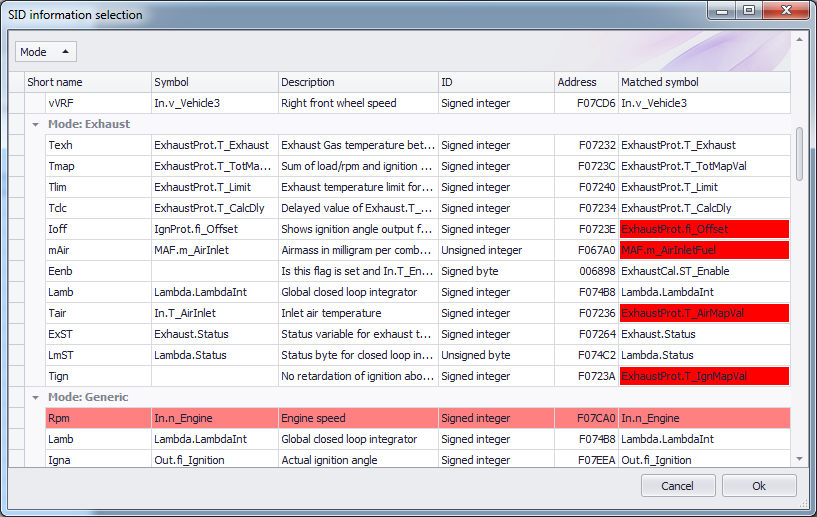
\includegraphics[width=.9\linewidth]{sid.png}
    \caption{SID Information}
    \label{fig:}
\end{figure}

Some tips on how to use the SID information option:
\begin{itemize}
    \item
        \texttt{ECMStat.ST\_ActiveAirDem} shows the current Airmass limiter.
    \item
        \texttt{ECMStat.P\_Engine} shows calculated engine power in horsepower.
    \item
        \texttt{ECMStat.AirFuelRatio} shows calculated AFR.
    \item
        \texttt{ECMStat.p\_Diff} shows boost pressure (manifold – ambient) in
        \SI{0.1}{\kilo\pascal} units.
    \item
        \texttt{BstKnkProt.MapPointer} shows the offset in \SI{0.1}{\degree} for
        \texttt{BstKnk.MaxAirmass} (so, the
        ignition offset for knock)
    \item
        \texttt{ExhaustCal.ST\_Enable} allows you to enable and disable the EGT
        algorithm. These algorithms are based on the stock engine and won’t be
        properly calibrated for a stage 3+ setup.
    \item
        \texttt{KnkDetAdap.KnkCntCyl} first 2 bytes show cylinder 1 knock count,
        next 2 bytes shows cylinder 2 knock count etc.
\end{itemize}

\chapter{CAN bus interface}
The most common way to interface with the Trionic 7 unit is via the CAN
bus\index{CAN}.

\section{General information}
\begin{table}
    \centering
    \begin{tabular}{ll}
        CAN controller & \texttt{ Intel AN825257} \\
        Communication speed & \SI{615}{\kilo\bit\per\second}
    \end{tabular}
    \caption{CAN specifications for Trionic 7}
    \label{tab:}
\end{table}
The most frequently used interface for this is the Lawicel CANUSB
interface\footnote{www.canusb.com}. This interface can convert CAN signals onto
you USB port and vice versa. The interface has a USB port on one side – that
connects to you computer – and an male \texttt{DB9} connector on the other side.
This side connects to the CAN bus of the Trionic.

The Lawicel interface has the
following pin out on the DB9 connector.
\Mfig{DB9}

\Mfig{Desk connection to ecu}


\section{Saab I-bus communication}
Courtesy of Tomili and General Failure

The I-Bus is an internal bus (Instrumentation Bus) that connects together
instruments such as the radio, ACC and the SID (Information Display). The I-bus
is the non-critical bus which means that vehicle critical information is not
sent over it. That is done through the P (powertrain) bus. The I-bus enables us
to communicate with several devices in the car including the TWICE, DICE etc.
Both the I and the P bus are CAN bus based communication buses which enables us
to use a normal CAN adapter to interface with them.

The I bus follows the ISO 11898-2 standard which is the high speed variant,
although it only implements a maximum communication speed of
\SI{47,619}{\kilo\bit\per\second}.
Messages on a CAN bus are sent within CAN frames that include an identifier
number, number of data bytes, the actual data (called the payload) and checksum
(to verify it the data was transferred correctly). There are two CAN frame
formats: the basic frame (referred to as CAN2.0A) and the extended frame
(referred to as CAN2.0B). The basic frame has a 11-bit identifier field, when
the extended frame has a 29-bit identifier which makes it possible to extend the
number of message types that can be sent over the bus. The I bus uses two signal
(just like any other CAN bus connection) which are called I+ and I-. These refer
to CAN High and CAN Low signals in general CAN terminology. Details on I bus
communication:

\begin{table}
    \centering
    \begin{tabular}{ll}

Frame type & CAN 2.0A (11-bit identifiers) \\
Bus speed & \SI{47,619}{\kilo\bit\per\second} \\
Timing register settings & BTR0 0xCB, BTR1 0x9A
    \end{tabular}
    \caption{}
    \label{tab:}
\end{table}

As an example the engine speed is located as a 16-bit integer value on message
ID 460h (hexadecimal) in the second and third bytes (I define first byte as the
most significant byte). Speed is in the same message in fourth and fifth bytes.
The speed value is multiplied by ten, so you have to divide the 16-bit integer
by 10 to get the real speed value.

Here's an example ID 460h message: \texttt{00 03 9C 00 2A 00 00 00}
Engine rpm is \texttt{039Ch} (hexadecimal format) = 924 (decimal format) =
\SI{942}{\rpm}. Speed is \texttt{002Ah} = 42 = \SI{4,2}{\kilo\meter\per\hour}.

\section{Trionic Data Initialization (220h)}
This message (\cref{tab:220h}) must be sent before any queries to the Trionic
can be sent. Trionic responds with a 238h message.
\begin{table}
    \centering
    \begin{tabular}{lllllllll}
        ID & Byte 0 & Byte 1 & Byte 2 & Byte 3 & Byte 4 & Byte 5 & Byte 6 & Byte 7 \\
        \midrule
        \texttt {220h} & \texttt{3Fh} & \texttt{81h} & \texttt{01h} & \texttt{33h} &
        \texttt{02h} & \texttt{40h} & \texttt{00h}& \texttt{00h}
    \end{tabular}
    \caption{220h Trionic Data Initialization}
    \label{tab:220h}
\end{table}

\section{Trionic Data Initialization Acknowledgement (238h)}
Trionic sends this message (\cref{tab:238h}) after a 220h message has been sent on the bus.
\begin{table}
    \centering
    \begin{tabular}{lllllllll}
        ID & Byte 0 & Byte 1 & Byte 2 & Byte 3 & Byte 4 & Byte 5 & Byte 6 & Byte 7 \\
        \midrule
        \texttt {238h} & \texttt{40h} & \texttt{BFh} & \texttt{21h} & \texttt{C1h} &
        \texttt{01h} & \texttt{11h} & \texttt{02h}& \texttt{58h}
    \end{tabular}
    \caption{238h Trionic Data Initialization Acknowledgement}
    \label{tab:238h}
\end{table}

\section{Trionic Data Query (240h)}
This message is sent as a command to the Trionic. It can be used to query
\enquote{OBD2} information. I use the quotation marks because basically this
information is also available from the OBD2 interface. The problem with the
OBD2 interface is that it's slow. By using directly the I-Bus (or even better,
the P-Bus) you can achieve refresh rates of \SIrange{10}{50}{\hertz}. The
\texttt{DATA} byte below
indicates what data is requested. The COMMAND byte is \texttt{01h} for requesting
OBD2 information. With \texttt{COMMAND} byte \texttt{1Ah} you can request information
from the Trionic software header. The header comprises of ASCII and
hexadecimal data about e.g. Vehicle Identification Number (VIN), Immobilizer
code, Software Saab part number, Hardware Saab part number and Software
version string.

The data query message is shown in \cref{tab:240h}. All known \texttt{DATA} values that can be queried is listen in
\cref{tab:trionic-data-01h}.

\begin{table}
    \centering
    \begin{tabular}{lllllllll}
        ID & Byte 0 & Byte 1 & Byte 2 & Byte 3 & Byte 4 & Byte 5 & Byte 6 & Byte 7 \\
        \midrule
        \texttt {240h} & \texttt{40h} & \texttt{A1h} & \texttt{02h} &
        \texttt{COMMAND} &
        \texttt{DATA} & \texttt{00h} & \texttt{00h}& \texttt{00h}
    \end{tabular}
    \caption{240h Trionic Data Query}
    \label{tab:240h}
\end{table}

\begin{table}
    \centering
    \begin{tabular}{lll}
        \texttt{DATA} & Description & How to handle reply value \\
        \midrule
        \texttt{00h} & Some generic request (requires more research) & ? \\
        \texttt{04h} & Calculated load value & unit is \\
        \texttt{05h} & Coolant temperature & subtract 40, unit \si{\degreeCelsius} \\
        \texttt{0Bh} & Manifold Air Pressure &MAP unit hPa \\
        \texttt{0Ch} & Engine RPM & Divide by 4, unit \si{\per\minute} \\
        \texttt{0Eh} & Engine timing advance & ? \\
        \texttt{0Fh} & Intake air temperature & subtract 40, unit \si{\degreeCelsius} \\
        \texttt{10h} & Mass Air Flow, MAF & divide by 100, unit \si{\gram\per\second} \\
        \texttt{14h} & O2 sensor 1, Bank 1 & ? \\
        \texttt{15h} & O2 sensor 2, Bank 1 & ? \\
    \end{tabular}
    \caption{All known \texttt{DATA} values that can be queries with
    \texttt{COMMAND} byte \texttt{01h}.}
    \label{tab:trionic-data-01h}
\end{table}


\todo{Finish I-bus and P-bus section}
\chapter{General tuning advice}
This chapter will describe some frequently made mistakes in handling the Trionic.
\begin{description}
    \item[Ignition advance]
        When altering the ignition tables keep in mind that more than 35 degree advance from TDC is not good.
    \item[Ignition retard]
        When altering the ignition tables keep in mind that more than 5 degreen retarding from TDC is not good.
    \item[Ignition advance at WOT] Try to keep the ignition advance at
        approximately 10 degrees BTDC
    \item[Recommended AFR] Try to keep the AFR between 10.8 and 12.5 at WOT.
    \item[Recommended EGT] Try to keep the exhaust gas temperature below 950
        degrees C.
    \item[Determining the maximum boost request for a given turbo] Check that the boost request level fits somehow to compressor map:
        \url{http://www.squirrelpf.com/turbocalc/index.php}\todo{Dead link!}
        In addition you can read appendix IV\todo{Internal link}.
    \item[Recommended maximum intake air temperature] Up to
        \SI{60}{\celsius} is good enough. If temperatures rise above
        \SI{60}{\celsius} consider replacing your stock
        intercooler with an aluminium, cross-flow type. These are available from Speedparts, Abbott, ETS and
        others.
\end{description}

\chapter{Tools}
\section{T7Suite}
T7Suite has the following features:
\begin{itemize}
    \item Checksum verification and correction
    \item Software ID adjustment
    \item Immobilizer code adjustment
    \item File comment adjustment
    \item Box number adjustment
    \item Extraction of symbol table
    \item Map visualization
    \item Compare maps in binary to another binary
    \item Move maps from one binary to another
    \item Downloading flash content from ECU through Canbus
    \item Flashing ECU through Canbus
    \item Real-time tuning (work in progress...)
\end{itemize}

For usage of this tool please refer to its user manual.

\section{BD32}
BD32.exe is the tool used to interface with the ECU through a BDM interface. It
is DOS based and will run normally on Win95/98/Me. Ideally the user would boot
into a DOS environment to use the tool. There is a windows version available but
the author has no experience with that specific tool.

\section{IDA Pro}
IDAPro stands for Interactive DisAssembler Professional. It enables the user to
disassemble binary files to its original source code. IDAPro is commercial
software, not freeware.

Example of how to use IDA Pro with a Trionic 7 box.
\begin{enumerate}
    \item Open binary/raw file
    \item Set processor to Motorola series: 68330
    \item Check the \texttt{Create RAM section}, start address 0xF00000, size 0xFFFF.
    \item Go to address ROM:00000000 in 'IDA View-A' and hit D-key three times
        to get dc.l \$FFFFEFFC
    \item Go to the next address ROM:00000004 and hit D-key three times to get reset vector address (this
        varies from binary to binary)
    \item You should get e.g. dc.l unk\_5169A or something like that, double-click
        the unk\_5169A text
    \item Your now in the place where the code execution starts, press C to disassemble
    \item Now, from the menu select Options -> General, go to Analysis tab and press
        \texttt{Kernel options1} button
    \item Check \texttt{Make final analysis pass} and hit OK
    \item Press \texttt{Reanalyze program} button and wait a while (this really takes some time, a minute or so)
\end{enumerate}

\section{Hex editor}
Hexworkshop (or UltraEdit) is a tool that comes in handy often. It can be used to view, search and
modify the raw binary file.

\appendix
\chapter{Symbol list}
This appendix will give a short description of the most important maps in
Trionic 7. To give a list of all symbols would be kind of stupid because there
are approximately 4000 (!!!) symbols in a Trionic 7 binary.

\begin{itemize}
    \item
        AirCtrlCal.m\_MaxAirTab
        Airmass value from controller where area map has reached max-area and there is no point to increase
        the I-part. Resolution is 1 mg/c.
    \item
        AirCtrlCal.m\_MaxAirE85Ta ( if running on E85 )
        Same as above for E85
    \item
        BoostCal.I\_LimTab
        Load limit tab. to enable the I Part of boost regulator. If the load request
        from Airmass master is above this value plus the hysteresis is the I Part
        enabled and the throttle closed loop is disabled. If the load request from
        Airmass master is below this value is the I Part disabled and the throttle is
        allowed to run in closed loop.
    \item
        BoostCal.P\_LimTab
        Load limit tab. to enable the P Part of boost regulator. If the load request
        from Airmass master is above this value plus the hysteresis is the P Part
        enabled. If the load request from Airmass master is below this value is the P
        Part disabled.
    \item
        BoostCal.RegMap
        Main constant matrix. Resolution is 0.1 %.
    \item
        BstKnkCal.MaxAirmass (divide by 3,1 for approx torque, ignition, airtemp etc
        affect this!) Map for max allowed Airmass for manual gearbox, m\_nHigh.
        Resolution is 1 mg/c.
\end{itemize}
\section{Knock limitation}
Knock control first retards the ignition timing for each cylinder. If the mean
value for the ignition retardation for all the cylinder exceeds a certain value,
fuel enrichment will take place. If the mean value for ignition retardation
increases further, the maximum permissible air mass per combustion will be
reduced with the values in the BstKnkCal.MaxAirmass maps. X axis represents
degree of ignition retard. This reduction takes place continuously as the
ignition retardation increases. The value constitutes the maximum air mass per
combustion value permitted by knock control.

Note: Knock control on modern engines is not a safety function but a normal
function. Consequently, it is considered normal when knock control reduces
engine torque in certain cases. The engine knock control increases for e.g. high
intake air temperatures or high coolant temperatures. Further influencing
factors are driving at high altitudes and low octane fuel. Certain engine
variants require fuel with an octane rating of \SI{98}{\RON} in order to provide the
specified engine torque and power.
\begin{itemize}
    \item
        BstKnkCal.MaxAirmassAu
        Map for max allowed Airmass for automatic gearbox, m\_nHigh. Resolution is 1 mg/c.
        See text above
    \item
        FCutCal.m\_AirInletLimit
        If the "MAF.m\_AirInletFuel" is higher than this limit during m\_AirInletTime will the fuelcut be activated
        ( pressure guard ).
    \item
        IgnE85Cal.fi\_AbsMap ( if you want to change the ignition )
        Ignition map for E85 fuel. Resolution is 0.1 °.
        IgnNormCal.Map ( if you want to change the ignition )
        Normal ignition map. Resolution is 0.1 °.
        MapChkCal.CheckSum (automatically updated in between every map change with T7suite!)
    \item
        MaxVehicCal.v\_MaxSpeed (max vehicle speed )
    \item
        PedalMapCal.m\_RequestMap
        Requested Airmass from the driver as a function of rpm and accelerator pedal position. Resolution is 1
        mg/c.
    \item
        TorqueCal.M\_ManGearLim
        Maximum engine torque limit for each gear in the manual gearbox. Resolution is 1 Nm.
        Manual gearbox, engine torque limitation
        The maximum engine torque must be limited at low gear ratios for reasons of strength.
        The control module calculates the engaged gear by comparing engine speed with vehicle speed.
        If the gear ratio corresponds with gear 1 or R, the control module reads bus information "Reverse
        gear selected" from DICE to distinguish between them.
        Engine torque is limited to:
        Gear 1 or R is limited to 230 Nm on engine alternative B205E/B235E. Engine torque is limited to 350
        Nm in other gears.
        On engine alternative B235E, gear 5 is gradually limited if the engine speed is below 2400 rpm. This is
        to avoid vibration.
        On engine alternative B235R, gear 1 is limited to 280 Nm and reverse gear, R, is limited to 230 Nm.
        Torque limitation in gears 2-5 is 380 Nm.
        The engine torque value is converted to \si{mgc} and constitutes the maximum air
        mass per combustion allowed by the gearbox.
    \item
        TorqueCal.m\_AirTorqMap This is where all torque limiters take their data from
        and therefore needs to be "fooled" if you are running more than
        \SI{400}{\newton\meter} or an automatic.
        The four-speed automatic need the last row to be max \SI{330}{\newton\meter},
        five-speed \SI{350}{\newton\meter}, as this is what the gearbox ECU is
        requesting as a max limit. Data-matrix for nominal Airmass. Engine speed and
        torque are used as support points. The value in the matrix + friction Airmass
        (idle Airmass) will create the pointed torque at the pointed engine speed.
        Resolution is 1 mg/c. axis to the above map: TorqueCal.m\_AirXSP
    \item
        TorqueCal.M\_EngMaxTab
        Data-table for maximum engine output torque for manual cars. Resolution is 1 Nm.
    \item
        TorqueCal.M\_EngMaxAutTab
        Data-table for maximum engine output torque for automatic cars. Resolution is 1 Nm.
        TCM, engine torque limitation
        The maximum engine torque must be limited in gear R, 1 and 2 for reasons of strength. TCM will send
        continuous bus information specifying the maximum permissible engine torque. The maximum
        permitted engine torque is also limited during gear changing. TCM sends maximum permissible engine
        speed:
        \begin{table}
            \centering
            \begin{tabular}{ll}
                Reverse & \SI{270}{\newton\meter} \\
                1st & \SI{330}{\newton\meter} \\
                2nd & \SI{330}{\newton\meter} \\
                3rd & \SI{330}{\newton\meter} \\
                4th & \SI{350}{\newton\meter} \\
                5th & \SI{350}{\newton\meter}
            \end{tabular}
            \caption{}
            \label{tab:}
        \end{table}
        TCM then sends maximum permissible engine torque to protect the gearbox.
        Trionic T7 converts \si{\newton\meter} to \si{\mgc} with help of the Airtorque map. The value constitutes
        the maximum air mass/combustion permitted by the automatic transmission and it is therefore we
        currently need to trick T7 to think more Airmass is still the same Nm.
    \item
        TorqueCal.M\_5GearLimTab
        Data-table for maximum engine output torque for manual cars on fifth gear.
        Resolution is \SI{1}{\newton\meter}.
    \item
        TorqueCal.M\_EngMaxE85Tab ( if running on E85 )
        Data-table for maximum engine output torque when running on E85. Resolution is
        \SI{1}{\newton\meter}.
    \item
        TorqueCal.m\_PedYSP
        Air mass support points for (Calc) X\_AccPedalMap. Resolution is 1 \si{\mgc}.
\end{itemize}

\chapter{Pinout diagrams}
Interfacing with the Trionic T7 unit through the CAN bus is possible

Chip used on Trionic side: Intel AN825257
Communication speed used: \SI{615}{\kilo\bit\per\second}.

The most frequently used interface for this is the Lawicel CANUSB interface that can be found on
www.canusb.com. This interface can convert CAN signals onto you USB port and vice versa. The
interface has a USB port on one side – that connects to you computer – and an male RS232 (DB9)
connector on the other side. This side connects to the CAN bus of the Trionic.

\begin{figure}[]
    \centering
    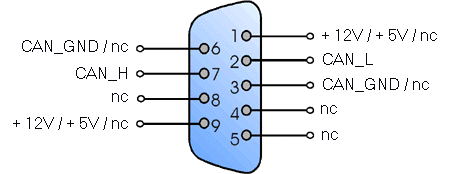
\includegraphics[width=\linewidth]{db9-pinout.png}
    \caption{}
    \label{fig:}
\end{figure}
\begin{figure}[]
    \centering
    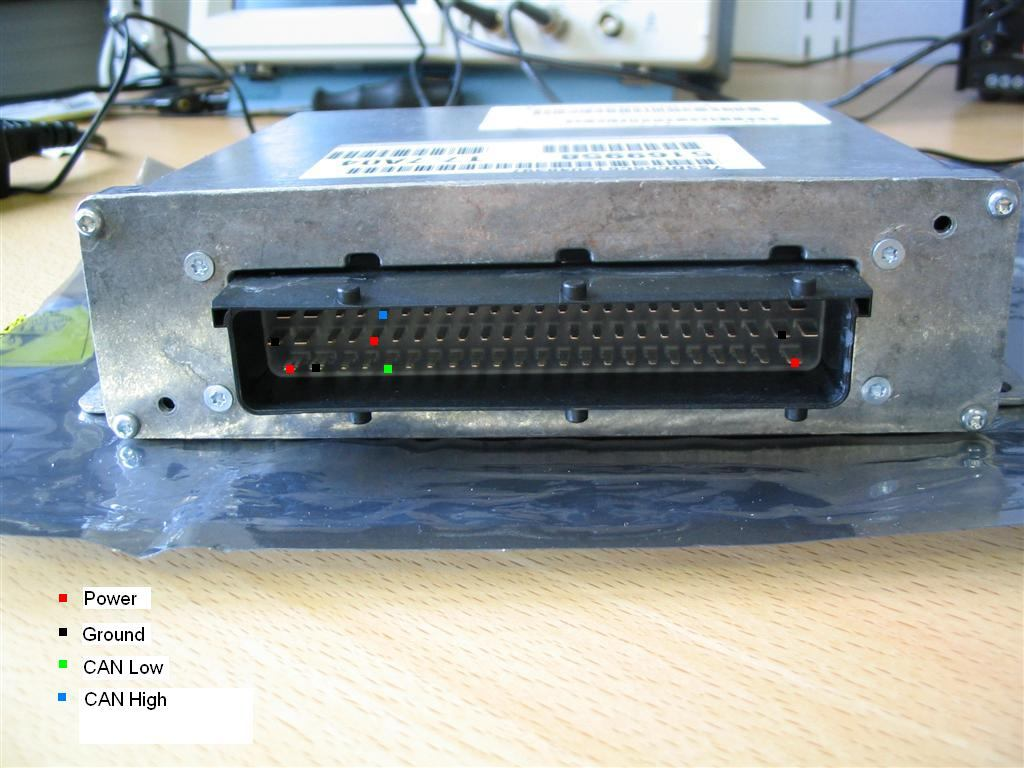
\includegraphics[width=\linewidth]{t7pinout.png}
    \caption{}
    \label{fig:}
\end{figure}

\section{OBD2 socket pinout}
\todo{Section should be updated with p-bus obd2 information}On some models, the
OBDII port enables you to connect to the I bus directly. On most models, you
need to wire into the P-pus (preferably, because data transmission rates are
tenfold of that on the Ibus) or into the I-bus directly. The P-bus can be found
at the pins of the ECU (as described on the previous page), the I-bus can be
found in a lot of places like the CD changer connector in the trunk (other spots
are shown in the table below).

\begin{table}
    \centering
    \begin{tabular}{ll}
        Pin number & Description \\
        \midrule
        1 & \\
        2 & J1850 Bus+ \\
        3 & \\
        4 & Chassis ground\\
        5 & Signal ground\\
        6 & CAN High (J-2284)\tablefootnote{Only on some models}\\
        7 & ISO 9141-2 K-line\\
        8 & \\
        9 & \\
        10 & J1850 Bus-\\
        11 & Airbag Controller (?)\\
        12 & ABS Controller (?)\\
        13 & \\
        14 & CAN Low (J-2284)\tablefootnote{Only on some models}\\
        15 & ISO 9141-2 L-line\\
        16 & Battery Power
    \end{tabular}
    \caption{}
    \label{tab:}
\end{table}

\chapter{BDM Technical Information}
BDM stands for Background Debug Mode. This refers to the mode the Motorola
microcontroller is forced into when activating the BDM interface. This mode
enables us to hold the processor in the program execution and read and write
data from and to the memory inside the microcontroller and the memory connected
to it. In this way we can download and program the flash contents which gives us
access to the binaries we like so much! The BDM software you need can be
downloaded from http://www.xendus.se/bdm/bd32-122.zip.

\section{Home build 2 chips design schema}
An alternative to buying a BDM interface can be building one yourself. This chapter will hand you all
information needed to buy the components needed and the schema to build the interface. The image
below shows the schema for the 2 chip design. There is also a 5 chip design and a GAL based design
but these are more difficult to build at home.

\Mfig{bdm-adapter}

\Cref{tab:bdm-part-list} lists the components you need to build the BDM interface. Of course a soldering
iron, PCB etc. are things that you also need.

\begin{table}
    \centering
    \begin{tabular}{lll}
        Component & Amount & Description \\
        \midrule
        74HC74 & 1 & Dual JK Flip-Flop with Set and Reset \\
        74HC132 & 1&  Quad 2-input NAND Schmitt Trigger \\
        Capacitor &0.1 uF& 1 \\
        Capacitor &0.001 uF& 1 \\
        Resistor &10 kohm & 1 \\
        LPT cable + connector &1 meter& Smart is to get PCB type with normal LPT cable.
        \\
        10 wire flat cable &20 cm  & \\
        10 pin female header for flat cable & 1
    \end{tabular}
    \caption{DIY BDM interface part list}
    \label{tab:bdm-part-list}
\end{table}

\section{BDM Pinout}
\begin{table}
    \centering
    \begin{tabular}{lll}
        Pin &  Name &  Description  \\
        \midrule
        1 &DS & Data strobe from target MCU. Not used
        in current interface circuitry \\
        2 &BERR &
        Bus error input to target. Allows
        development system to force bus error
        when target MCU accesses invalid
        memory \\
        3 &VSS & Ground reference from target \\
        4 &BKPT/DSCLK &
        Breakpoint input to target in normal
        mode; development serial clock in
        BDM. Must be held low on rising edge
        of reset to enable BDM \\
        5 &VSS & Ground reference from target \\
        6 &FREEZE & Freeze signal from target. High level
        indicates that target is in BDM \\
        7 &RESET & Reset signal to/from target. Must be
        held low to force hardware reset \\
        8 &IFETCH/DSI &
        Used to track instruction pipe in normal
        mode. Serial data input to target MCU
        in BDM \\
        9 &VCC &
        +5V supply from target.BDM interface
        circuit draws power from this supply
        and also monitors 'target powered/not
        powered' status \\
        10 &IPIPE/DSO &
        Tracks instruction pipe in normal mode.
        Serial data output from target MCU in
        BDM
    \end{tabular}
    \caption{}
    \label{tab:}
\end{table}

\chapter{Understanding turbo compressor maps}
Each turbo has its own characteristics. These are determined by the size of the turbine housing, the
size of the compressor wheel, the size of the turbine blades and many more parameters.
The most important identification of a turbocharger is by its compressor map. This is a graphical
representation of its efficiency. In Saab Trionic 7 cars there are two commonly
used turbo chargers; the
Garrett GT17 for all models except for B205R and B235R. These latter engines are
instead equipped with the Mitsubishi TD04-HL-15T (6cm2).

For an introduction to turbocharger terminology and concepts, please
see~\textcite{GarrettTerminology}. For information on basic flow calculation and how
to choose between turbochargers, see~\textcite{Isaac-Lowry2004}.
\begin{itemize}
    \item Compressor and turbine wheels. The turbine wheel is the vaned wheel
        that is in the exhaust gases from the engine. It is propelled by the
        exhaust gases themselves. The turbine wheel is connected to the
        compressor wheel by an axle. So, the compressor wheel will spin together
        with the turbine wheel. The compressor wheel also is vaned and these
        vanes compress the air and force it into the intercooler.
    \item Wheel “trim”. Trim is an area ratio used to describe both turbine and
        compressor wheels. Trim is calculated using the inducer and exducer
        diameters. As trim is increased, the wheel can support more air/gas flow.
    \item Compressor and turbine housing A/R. A/R describes a geometric property of
        all compressor and turbine housings. Increasing compressor A/R optimizes the
        performance for low boost applications. Changing turbine A/R has many
        effects. By going to a larger turbine A/R, the turbo comes up on boost at a
        higher engine speed, the flow capacity of the turbine is increased and less
        flow is wastegated, there is less engine backpressure, and engine volumetric
        efficiency is increased resulting in more overall power.
    \item Clipping. When an angle is machined on the turbine wheel exducer (outlet
        side), the wheel is said to be 'clipped'. Clipping causes a minor increase
        in the wheel's flow capability, however, it dramatically lowers the turbo
        efficiency. This reduction causes the turbo to come up on boost at a
        later engine speed (increased turbo lag). High performance applications
        should never use a clipped turbine wheel. All Garrett GT turbos use
        modern unclipped wheels.
    \item CFM = Cubic feet per minute.
    \item Lbs/minute = pounds (weight) per minute.
    \item M3/s = cubic meters per second.
    \item Corrected Airflow. Represents the corrected mass flow rate of air,
        taking into account air density (ambient temperature and pressure)

        \begin{definition}
            The corrected airflow $C_{corr}$ is defined as
            \begin{equation}
                C_{corr}=C_{air}\frac{13.95}{P}\sqrt{\frac{T_{air} +460}{545}}
            \end{equation}
            where \todo{We should only use SI units}$T_{air}$ is the air temperature in Fahrenheit, $P$ the barometric pressure in
            psi, and $C_{air}$ the
            engine air consumption in lb/min.
            \label{def:corrected-airflow}
        \end{definition}
        \begin{example}
            With $T_{air}=60 F$, $P=14.7$ psi and $C_{air}=50$ lb/min we get
            \begin{equation}
                C_{corr}=50\frac{13.95}{14.7}\sqrt{\frac{60+460}{545}}=46.3\text{
                lb/min}
            \end{equation}
            \label{ex:corrected-airflow}
        \end{example}
    \item Pressure ratio. Ratio of absolute outlet pressure divided by absolute
        inlet pressure.
        \begin{definition}
            The pressure ratio $R_{pressure}$ is defined as
            \begin{equation}
                R_{pressure}=\frac{P_{boost}+P_{IC}+P_0}{P_0-P_{AF}}
            \end{equation}
            where $P_{boost}$ is the intake manifold pressure
            (boost\index{Boost}) in psi, $P_{IC}$ is the intercooler pressure
            drop in psi,
            $DP_{AF}$ the air filter pressure drop in psi and $P_0$ is the air pressure
            at sea level in psi.
            \label{}
        \end{definition}
        \begin{example}
            With $P_{boost}=12$ psi, $P_{IC}=2$ psi, $P_{AF}=0.5$ psi and
            $P_0=14.7$ psi we get
            \begin{equation}
                R_{pressure}=\frac{12+2+14.7}{14.7-0.5}=2.02
                \label{}
            \end{equation}

        \end{example}
\end{itemize}
\section{Reading a compressor map}
This section contains a short description of reading compressor maps. For a more
detailed analysis, see
\textcite{Isaac-Lowry2004}. A 2-dimensional pressure map looks like this.
\Mfig{Compressor map}


The curved lines indicate the rotation speed (rpm) of the compressor wheel. In the sample map
above these values are 45050, 69750, 84200 up to 125650 rpm. This is how fast a turbine wheel
spins!!
The elliptical circle means the compressor's efficiency area. It's marked by the percent sign.
The horizontal axis is the amount of air before turbo, (1 m3/s = 2118.88 cfm, 10 lb/min = 144.718
cfm).

The vertical axis is the pressure ratio, the ratio of air pressure leaving to the turbo to air pressure
entering the turbo.
Pressure Ratio=The pressure at compressor exducer vs. the pressure at compressor inducer.
In another word, the ratio of the pressure of the air after compression vs. the pressure before
compression. As you can see, the pressure ratio depends on the ambient pressure. For example, at
sea level, a turbo boosts 14.7psi. Ambient pressure is 14.7psi. That's 2 pressure ratio (PR) on the
compressor map. Take that turbo to a higher elevation, the ambient pressure is less than 14.7psi. If
the turbo still boosts 14.7psi, the pressure ratio would be higher. Now on the compressor map, you
will see by moving up along a vertical line (to pump out the same cfm) and turbo efficiency has
decreased as the elevation increases (PR increases). Simply put, turbos lose performance and become
less efficient as elevation gets higher.

\subsection{Choke area}
The area to the right of the outer most elliptical circle is the least efficient area, the choke area.
It means when the compressor reaches certain rpm, the air moved by the compressor wheel in the
diffuser area of the compressor housing is moving at or past the speed of sound. When the air speed
reach sonic speed, the amount of air flow increase is very small as compressor wheel rpm increases.
In plain words, the compressor has reached its limit. You can try to pump more psi, have the wheel
spin faster, but very little more air is pumped out the turbo compressor. You can see now, the
compressor housing will need to properly match the compressor wheel. If you simply stuff a big wheel
inside a small compressor housing, the diffuse area will be very small. This causes the air inside the
housing to move at higher speed. That's why some of the so-called T28s which use a bigger
compressor wheel inside the stock compressor housing does not produce good hp.

\subsection{Compressor maximum flow}
The max flow of a compressor is shown on the compressor map. On the map, look for the intersection
of maximum compressor wheel speed (rpm) and the least compressor efficiency curve. Find that
intersection. The horizontal coordinate is the max flow.
The area to the right of maximum flow is the 'choke area'.

The vertical coordinate is the pressure ratio at which the compressor reaches that maximum flow.
From this boost level, as the boost increases, very little air flow is increased. For example, if a
compressor reaches its maximum flow at 2 PR or 1 atm pressure or 14.7psi, higher boost does not
pump more air into the motor. But higher boost may be needed to increase the manifold pressure for
the motor to flow more air. A 5 liter motor with this turbo needs 15psi of manifold pressure to flow a
certain CFM. A 3 liter motor with the same turbo will need much higher manifold pressure to flow the
same amount of air although that turbo's compressor does not flow more air past 14.7psi.

\subsection{Compressor maximum pressure}
On the map, find the top-most point on the graph. The vertical coordinate is the max pressure ratio.
For example, 2.8 pressure ratio at sea level is 1.8 times the atmospheric pressure, 1.8x14.7psi=26.46
psi. Compressor max pressure is limited by compressor wheel speed. It's physically impossible to
boost higher than this maximum pressure for one particular turbo. Plus the pressure drop in the
intercooler system, the actual maximum boost reading from a boost gauge that's plugged into the
intake manifolds maybe a few psi lower than this maximum pressure.

\subsection{What the compressor map reads}
Most manufactures rate their turbos at 1 bar (15 psi). That's 2 pressure ratio. On the map, draw a
horizontal line from 2PR. When the line intersects the right-most elliptical circle, the corresponding
number on the x-axis is the maximum cfm the turbo can flow at 1 bar.
Use the TD04-15G's map for example, where the 2 PR line hits the right-most efficiency curve, it
reads 428cfm as its flow rate at 15psi.

\subsection{Comparing compressor maps}
Well, compressor maps are really 3-dimensional maps. Any compressor map looks a hill/peak in 3
dimensions. Our compressor maps look like if you look at the hill directly from above vertically. The
elliptical lines of elevations are the efficiency curves. Since in theory, we can always boost more and
decrease turbo efficiency to get more cfm, let’s set the same Pressure Ratio and compare turbos at
the same efficiency curves.

As a rule of thumb, a large turbo will be better at making a lot of pressure but will spool slower than a
small turbo. A small turbo will build boost fast but is less capable to make big boost pressure.

\section{Selecting a different turbocharger}
In order to put in a new turbocharger we first need some
theory~\cite{Isaac-Lowry2004}.
\begin{definition}
    The engine volumetric
    flow\index{Engine Volumetric Flow} ($H$) in cfm \todo{imperial warning}is defined as
    \begin{equation}
        H=\frac{D_{ci}}{1728}\times\frac{n}{2}
        \label{eqn:volumetric-flow}
    \end{equation}
    where $D_{ci}$ is the engine displacement in cubic inches and $n$ is the number
    of crankshaft revolutions per minute.
    \label{}
\end{definition}
We can then find the airflow in lb/min by computing~\cite{Isaac-Lowry2004}.
\begin{equation}
    N=\frac{29PH}{10.73T}
    \label{eqn:airflow}
\end{equation}
where $P$ is the absolute pressure in psi and $T$ is the absolute ambient
temperature in Rankin.

\Cref{tab:volumetric-flow-rpm,tab:airflow-rpm}The following tables apply to our Saab 2.0 and 2.3 liter engines\todo{must
convert to metric}.
\begin{table}
    \centering
    \begin{tabular}{lll}
        RPM & 2.0L & 2.3L \\
        \midrule
        1000 & 35.3 &40.6 \\
        2000 & 70.6 &81.2  \\
        3000 & 105.9 &121.8 \\
        4000 & 141.3 &162.4 \\
        5000 & 176.6 &203.1 \\
        6000 & 211.9 &243.7 \\
        7000 & 247.2 &284.3
    \end{tabular}
    \caption{Engine volumetric flow ($H$) in cfm as given by \cref{eqn:volumetric-flow}
    for different rpm.}
    \label{tab:volumetric-flow-rpm}
\end{table}
Since the amount of air to be flowed by the turbo is largest when RPM is at its
top we will take the worst case scenario and get EVF @ 7000 RPM. We have to make
an assumption on the ambient temperature which we will set at 20C. This is 68
Fahrenheit which is (460 + 68) = 528 Rankin. Now we can calculate the airflow of
the engine in lb/min for any given boost level. If we want to draw a line into
the compressor map for our engines needs we need to calculate the needed airflow
for several boost levels.

\begin{table}
    \centering
    \begin{tabular}{llllll}
        Boost (bar) & Boost (psi) & 2.0L lb/min & 2.0L cfm & 2.3L lb/min & 2.3L
        cfm \\
        \midrule
        0.2 & 2.9 &3.7& 53.1& 4.2& 61 \\
        0.4 & 5.8 &7.3 &106.1& 8.4& 122 \\
        0.6 & 8.7 &11& 159.2 &12.6 &183 \\
        0.8 & 11.6& 14.7& 212.2 &16.9 &244 \\
        1.0 & 14.5& 18.3& 265.3 &21.1 &305 \\
        1.2 & 17.4& 22& 318.3 &25.3 &366 \\
        1.4 & 20.3& 25.7 &371.4 &29.5 &427 \\
        1.6 & 23.2& 29.3 &424.4 &33.8 & 488
    \end{tabular}
    \caption{Airflow in cfm and lb/min as given by \cref{eqn:airflow}}
    \label{tab:airflow-rpm}
\end{table}

This all results in 2 simple lines in the compressor map which indicate the maximum flow required
from the turbo by our engine.
\Mfig{turbo-lines}
Now we can clearly see where out engine leaves the compressor map and thus the limit for the
combination of the two (engine and turbo) lies.
We also see that – even for the 2.3 litre engine – the TD04 can sustain a much higher boost pressure
at higher rpms than the T25 can. Even at 1.4 bar boost (pressure ratio = 2.4) the TD04 is within its
limits and would flow approximately 420 cfm. Would we have done the same with the T25 turbo we
would most certainly be in the choke area and the turbo would be unable to get us the airflow that we
required.

For selecting the best wheel trim-housing, see~\cite{Isaac-Lowry2004}.

\section{Conclusion}
Comparing the two compressor maps for TD04 and T25 (see \cref{chap:turbo-specs})
we can clearly see that the TD04 can flow more air at a higher pressure ratio
and with a higher efficiency. Given the fact that the turbine blades are larger
than in the T25, spool up will be a bit slower, but high end power will be much
better. Upgrading your turbo will affect more than meets the eye. The VE map in
the Trionic would probably need adjustments because the hardware in the airflow
has been changed. This means the volumetric efficiency also changes and thus the
correction table needs changing too. Also, when boost values rise, the
intercoolers capacity for air flow comes into play. You must make sure that the
intercooler is not so restrictive that upgrading the turbo will result in a
burst intercooler. A high capacity cross flow intercooler would be a good option
here. And last but not least, upgrading the turbo charger means – that is the
goal here – more air flow to the cylinders and thus more oxygen to burn. If we
upgrade the turbo we need to consider the injectors too. If the injectors can’t
flow the amount of fuel needed to burn the amount of oxygen pushed into the
cylinders we would have gained nothing.

\chapter{Specifications of common Saab turbochargers}\label{chap:turbo-specs}
\todo{Needs the GT17}
\todo{Import from pdf}

\chapter{Sensors and actuators}
This appendix will list details about the sensors and actuators used in a T7 car.

Sensors are devices used to gather information. In a Trionic 7 car a lot of
sensors are used to determine what actions to take inside the ECU. These sensors
are all analogue, which means they output a signal that has to be converted to
digital numbers for the ECU to be able to understand them. Actuators on the
other hand are devices that enable the ECU to interact with the processes in the
car. Actuators are driven (or activated) by the Trionic be it directly or
indirectly.

\chapter{Connecting BDM interface to ECU}
\Mfig{BDM pinout}
\todo{Write this chapter, take note that Trionic7.pdf has incorrect info (see
github issue)}

Video guide: \url{https://www.youtube.com/watch?v=6FeAxgASqg4}

\printindex

\printbibliography

\end{document}
